% Created by tikzDevice version 0.12 on 2019-08-06 21:01:05
% !TEX encoding = UTF-8 Unicode
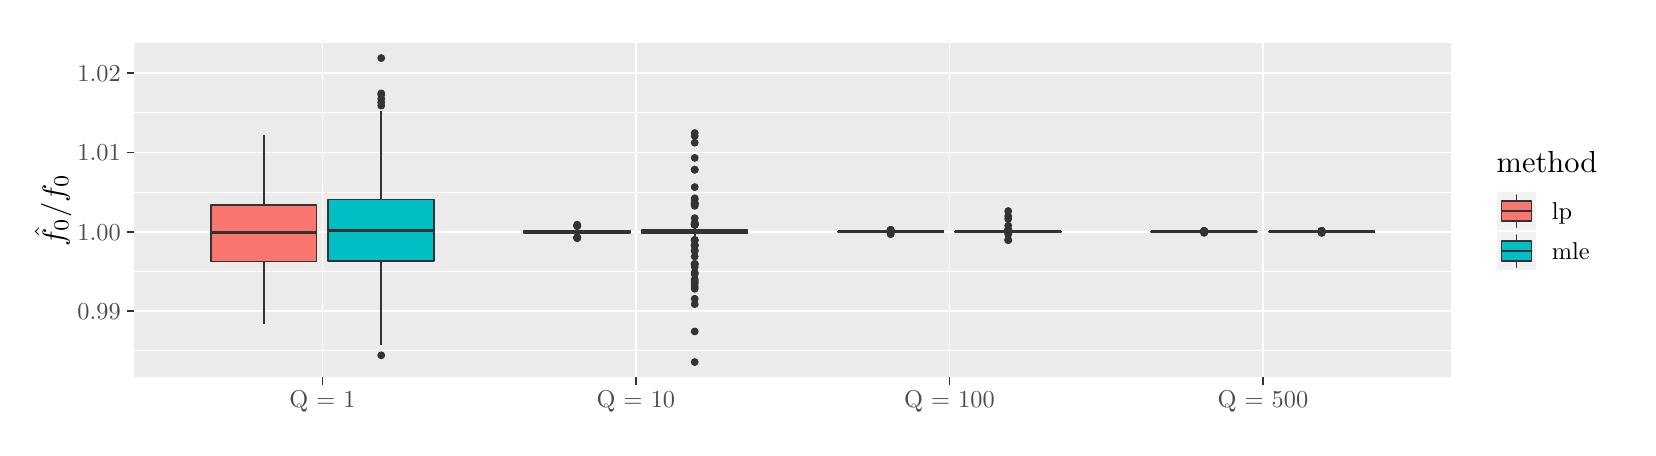
\begin{tikzpicture}[x=1pt,y=1pt]
\definecolor{fillColor}{RGB}{255,255,255}
\path[use as bounding box,fill=fillColor,fill opacity=0.00] (0,0) rectangle (578.16,144.54);
\begin{scope}
\path[clip] (  0.00,  0.00) rectangle (578.16,144.54);
\definecolor{drawColor}{RGB}{255,255,255}
\definecolor{fillColor}{RGB}{255,255,255}

\path[draw=drawColor,line width= 0.6pt,line join=round,line cap=round,fill=fillColor] (  0.00,  0.00) rectangle (578.16,144.54);
\end{scope}
\begin{scope}
\path[clip] ( 38.56, 18.22) rectangle (514.31,139.04);
\definecolor{fillColor}{gray}{0.92}

\path[fill=fillColor] ( 38.56, 18.22) rectangle (514.31,139.04);
\definecolor{drawColor}{RGB}{255,255,255}

\path[draw=drawColor,line width= 0.3pt,line join=round] ( 38.56, 27.80) --
	(514.31, 27.80);

\path[draw=drawColor,line width= 0.3pt,line join=round] ( 38.56, 56.45) --
	(514.31, 56.45);

\path[draw=drawColor,line width= 0.3pt,line join=round] ( 38.56, 85.10) --
	(514.31, 85.10);

\path[draw=drawColor,line width= 0.3pt,line join=round] ( 38.56,113.74) --
	(514.31,113.74);

\path[draw=drawColor,line width= 0.6pt,line join=round] ( 38.56, 42.13) --
	(514.31, 42.13);

\path[draw=drawColor,line width= 0.6pt,line join=round] ( 38.56, 70.77) --
	(514.31, 70.77);

\path[draw=drawColor,line width= 0.6pt,line join=round] ( 38.56, 99.42) --
	(514.31, 99.42);

\path[draw=drawColor,line width= 0.6pt,line join=round] ( 38.56,128.07) --
	(514.31,128.07);

\path[draw=drawColor,line width= 0.6pt,line join=round] (106.52, 18.22) --
	(106.52,139.04);

\path[draw=drawColor,line width= 0.6pt,line join=round] (219.79, 18.22) --
	(219.79,139.04);

\path[draw=drawColor,line width= 0.6pt,line join=round] (333.07, 18.22) --
	(333.07,139.04);

\path[draw=drawColor,line width= 0.6pt,line join=round] (446.34, 18.22) --
	(446.34,139.04);
\definecolor{drawColor}{gray}{0.20}

\path[draw=drawColor,line width= 0.6pt,line join=round] ( 85.28, 80.47) -- ( 85.28,105.71);

\path[draw=drawColor,line width= 0.6pt,line join=round] ( 85.28, 60.00) -- ( 85.28, 37.48);
\definecolor{fillColor}{RGB}{248,118,109}

\path[draw=drawColor,line width= 0.6pt,line join=round,line cap=round,fill=fillColor] ( 66.17, 80.47) --
	( 66.17, 60.00) --
	(104.40, 60.00) --
	(104.40, 80.47) --
	( 66.17, 80.47) --
	cycle;

\path[draw=drawColor,line width= 1.1pt,line join=round] ( 66.17, 70.53) -- (104.40, 70.53);
\definecolor{fillColor}{gray}{0.20}

\path[draw=drawColor,line width= 0.4pt,line join=round,line cap=round,fill=fillColor] (127.76,116.37) circle (  1.21);

\path[draw=drawColor,line width= 0.4pt,line join=round,line cap=round,fill=fillColor] (127.76,118.82) circle (  1.21);

\path[draw=drawColor,line width= 0.4pt,line join=round,line cap=round,fill=fillColor] (127.76, 26.15) circle (  1.21);

\path[draw=drawColor,line width= 0.4pt,line join=round,line cap=round,fill=fillColor] (127.76,120.23) circle (  1.21);

\path[draw=drawColor,line width= 0.4pt,line join=round,line cap=round,fill=fillColor] (127.76,120.79) circle (  1.21);

\path[draw=drawColor,line width= 0.4pt,line join=round,line cap=round,fill=fillColor] (127.76,117.51) circle (  1.21);

\path[draw=drawColor,line width= 0.4pt,line join=round,line cap=round,fill=fillColor] (127.76,133.55) circle (  1.21);

\path[draw=drawColor,line width= 0.6pt,line join=round] (127.76, 82.39) -- (127.76,114.56);

\path[draw=drawColor,line width= 0.6pt,line join=round] (127.76, 60.28) -- (127.76, 29.73);
\definecolor{fillColor}{RGB}{0,191,196}

\path[draw=drawColor,line width= 0.6pt,line join=round,line cap=round,fill=fillColor] (108.64, 82.39) --
	(108.64, 60.28) --
	(146.87, 60.28) --
	(146.87, 82.39) --
	(108.64, 82.39) --
	cycle;

\path[draw=drawColor,line width= 1.1pt,line join=round] (108.64, 71.24) -- (146.87, 71.24);
\definecolor{fillColor}{gray}{0.20}

\path[draw=drawColor,line width= 0.4pt,line join=round,line cap=round,fill=fillColor] (198.56, 68.60) circle (  1.21);

\path[draw=drawColor,line width= 0.4pt,line join=round,line cap=round,fill=fillColor] (198.56, 72.82) circle (  1.21);

\path[draw=drawColor,line width= 0.4pt,line join=round,line cap=round,fill=fillColor] (198.56, 68.71) circle (  1.21);

\path[draw=drawColor,line width= 0.4pt,line join=round,line cap=round,fill=fillColor] (198.56, 72.93) circle (  1.21);

\path[draw=drawColor,line width= 0.4pt,line join=round,line cap=round,fill=fillColor] (198.56, 73.34) circle (  1.21);

\path[draw=drawColor,line width= 0.4pt,line join=round,line cap=round,fill=fillColor] (198.56, 68.77) circle (  1.21);

\path[draw=drawColor,line width= 0.4pt,line join=round,line cap=round,fill=fillColor] (198.56, 68.48) circle (  1.21);

\path[draw=drawColor,line width= 0.4pt,line join=round,line cap=round,fill=fillColor] (198.56, 72.97) circle (  1.21);

\path[draw=drawColor,line width= 0.4pt,line join=round,line cap=round,fill=fillColor] (198.56, 68.57) circle (  1.21);

\path[draw=drawColor,line width= 0.6pt,line join=round] (198.56, 71.24) -- (198.56, 72.62);

\path[draw=drawColor,line width= 0.6pt,line join=round] (198.56, 70.27) -- (198.56, 68.86);
\definecolor{fillColor}{RGB}{248,118,109}

\path[draw=drawColor,line width= 0.6pt,line join=round,line cap=round,fill=fillColor] (179.44, 71.24) --
	(179.44, 70.27) --
	(217.67, 70.27) --
	(217.67, 71.24) --
	(179.44, 71.24) --
	cycle;

\path[draw=drawColor,line width= 1.1pt,line join=round] (179.44, 70.76) -- (217.67, 70.76);
\definecolor{fillColor}{gray}{0.20}

\path[draw=drawColor,line width= 0.4pt,line join=round,line cap=round,fill=fillColor] (241.03,106.46) circle (  1.21);

\path[draw=drawColor,line width= 0.4pt,line join=round,line cap=round,fill=fillColor] (241.03, 97.48) circle (  1.21);

\path[draw=drawColor,line width= 0.4pt,line join=round,line cap=round,fill=fillColor] (241.03, 75.72) circle (  1.21);

\path[draw=drawColor,line width= 0.4pt,line join=round,line cap=round,fill=fillColor] (241.03, 93.22) circle (  1.21);

\path[draw=drawColor,line width= 0.4pt,line join=round,line cap=round,fill=fillColor] (241.03, 73.27) circle (  1.21);

\path[draw=drawColor,line width= 0.4pt,line join=round,line cap=round,fill=fillColor] (241.03, 82.47) circle (  1.21);

\path[draw=drawColor,line width= 0.4pt,line join=round,line cap=round,fill=fillColor] (241.03, 67.75) circle (  1.21);

\path[draw=drawColor,line width= 0.4pt,line join=round,line cap=round,fill=fillColor] (241.03, 93.21) circle (  1.21);

\path[draw=drawColor,line width= 0.4pt,line join=round,line cap=round,fill=fillColor] (241.03, 53.60) circle (  1.21);

\path[draw=drawColor,line width= 0.4pt,line join=round,line cap=round,fill=fillColor] (241.03, 53.07) circle (  1.21);

\path[draw=drawColor,line width= 0.4pt,line join=round,line cap=round,fill=fillColor] (241.03, 73.40) circle (  1.21);

\path[draw=drawColor,line width= 0.4pt,line join=round,line cap=round,fill=fillColor] (241.03, 73.69) circle (  1.21);

\path[draw=drawColor,line width= 0.4pt,line join=round,line cap=round,fill=fillColor] (241.03, 73.33) circle (  1.21);

\path[draw=drawColor,line width= 0.4pt,line join=round,line cap=round,fill=fillColor] (241.03, 81.31) circle (  1.21);

\path[draw=drawColor,line width= 0.4pt,line join=round,line cap=round,fill=fillColor] (241.03, 55.48) circle (  1.21);

\path[draw=drawColor,line width= 0.4pt,line join=round,line cap=round,fill=fillColor] (241.03, 67.76) circle (  1.21);

\path[draw=drawColor,line width= 0.4pt,line join=round,line cap=round,fill=fillColor] (241.03, 51.94) circle (  1.21);

\path[draw=drawColor,line width= 0.4pt,line join=round,line cap=round,fill=fillColor] (241.03, 73.43) circle (  1.21);

\path[draw=drawColor,line width= 0.4pt,line join=round,line cap=round,fill=fillColor] (241.03, 23.71) circle (  1.21);

\path[draw=drawColor,line width= 0.4pt,line join=round,line cap=round,fill=fillColor] (241.03, 59.04) circle (  1.21);

\path[draw=drawColor,line width= 0.4pt,line join=round,line cap=round,fill=fillColor] (241.03, 64.08) circle (  1.21);

\path[draw=drawColor,line width= 0.4pt,line join=round,line cap=round,fill=fillColor] (241.03, 44.64) circle (  1.21);

\path[draw=drawColor,line width= 0.4pt,line join=round,line cap=round,fill=fillColor] (241.03, 65.69) circle (  1.21);

\path[draw=drawColor,line width= 0.4pt,line join=round,line cap=round,fill=fillColor] (241.03, 61.86) circle (  1.21);

\path[draw=drawColor,line width= 0.4pt,line join=round,line cap=round,fill=fillColor] (241.03, 59.16) circle (  1.21);

\path[draw=drawColor,line width= 0.4pt,line join=round,line cap=round,fill=fillColor] (241.03, 56.04) circle (  1.21);

\path[draw=drawColor,line width= 0.4pt,line join=round,line cap=round,fill=fillColor] (241.03, 86.93) circle (  1.21);

\path[draw=drawColor,line width= 0.4pt,line join=round,line cap=round,fill=fillColor] (241.03,105.39) circle (  1.21);

\path[draw=drawColor,line width= 0.4pt,line join=round,line cap=round,fill=fillColor] (241.03, 50.19) circle (  1.21);

\path[draw=drawColor,line width= 0.4pt,line join=round,line cap=round,fill=fillColor] (241.03, 58.08) circle (  1.21);

\path[draw=drawColor,line width= 0.4pt,line join=round,line cap=round,fill=fillColor] (241.03, 63.86) circle (  1.21);

\path[draw=drawColor,line width= 0.4pt,line join=round,line cap=round,fill=fillColor] (241.03, 73.58) circle (  1.21);

\path[draw=drawColor,line width= 0.4pt,line join=round,line cap=round,fill=fillColor] (241.03,102.98) circle (  1.21);

\path[draw=drawColor,line width= 0.4pt,line join=round,line cap=round,fill=fillColor] (241.03, 74.05) circle (  1.21);

\path[draw=drawColor,line width= 0.4pt,line join=round,line cap=round,fill=fillColor] (241.03, 46.57) circle (  1.21);

\path[draw=drawColor,line width= 0.4pt,line join=round,line cap=round,fill=fillColor] (241.03, 80.72) circle (  1.21);

\path[draw=drawColor,line width= 0.4pt,line join=round,line cap=round,fill=fillColor] (241.03, 80.97) circle (  1.21);

\path[draw=drawColor,line width= 0.4pt,line join=round,line cap=round,fill=fillColor] (241.03, 82.88) circle (  1.21);

\path[draw=drawColor,line width= 0.4pt,line join=round,line cap=round,fill=fillColor] (241.03, 50.96) circle (  1.21);

\path[draw=drawColor,line width= 0.4pt,line join=round,line cap=round,fill=fillColor] (241.03, 80.89) circle (  1.21);

\path[draw=drawColor,line width= 0.4pt,line join=round,line cap=round,fill=fillColor] (241.03, 59.21) circle (  1.21);

\path[draw=drawColor,line width= 0.4pt,line join=round,line cap=round,fill=fillColor] (241.03, 73.35) circle (  1.21);

\path[draw=drawColor,line width= 0.4pt,line join=round,line cap=round,fill=fillColor] (241.03, 67.81) circle (  1.21);

\path[draw=drawColor,line width= 0.4pt,line join=round,line cap=round,fill=fillColor] (241.03, 66.00) circle (  1.21);

\path[draw=drawColor,line width= 0.4pt,line join=round,line cap=round,fill=fillColor] (241.03, 34.77) circle (  1.21);

\path[draw=drawColor,line width= 0.4pt,line join=round,line cap=round,fill=fillColor] (241.03, 65.84) circle (  1.21);

\path[draw=drawColor,line width= 0.4pt,line join=round,line cap=round,fill=fillColor] (241.03, 52.53) circle (  1.21);

\path[draw=drawColor,line width= 0.4pt,line join=round,line cap=round,fill=fillColor] (241.03, 65.90) circle (  1.21);

\path[draw=drawColor,line width= 0.4pt,line join=round,line cap=round,fill=fillColor] (241.03, 80.16) circle (  1.21);

\path[draw=drawColor,line width= 0.6pt,line join=round] (241.03, 71.32) -- (241.03, 73.02);

\path[draw=drawColor,line width= 0.6pt,line join=round] (241.03, 70.11) -- (241.03, 68.31);
\definecolor{fillColor}{RGB}{0,191,196}

\path[draw=drawColor,line width= 0.6pt,line join=round,line cap=round,fill=fillColor] (221.92, 71.32) --
	(221.92, 70.11) --
	(260.15, 70.11) --
	(260.15, 71.32) --
	(221.92, 71.32) --
	cycle;

\path[draw=drawColor,line width= 1.1pt,line join=round] (221.92, 70.75) -- (260.15, 70.75);
\definecolor{fillColor}{gray}{0.20}

\path[draw=drawColor,line width= 0.4pt,line join=round,line cap=round,fill=fillColor] (311.83, 70.19) circle (  1.21);

\path[draw=drawColor,line width= 0.4pt,line join=round,line cap=round,fill=fillColor] (311.83, 71.42) circle (  1.21);

\path[draw=drawColor,line width= 0.4pt,line join=round,line cap=round,fill=fillColor] (311.83, 69.90) circle (  1.21);

\path[draw=drawColor,line width= 0.4pt,line join=round,line cap=round,fill=fillColor] (311.83, 71.46) circle (  1.21);

\path[draw=drawColor,line width= 0.4pt,line join=round,line cap=round,fill=fillColor] (311.83, 71.42) circle (  1.21);

\path[draw=drawColor,line width= 0.6pt,line join=round] (311.83, 70.92) -- (311.83, 71.32);

\path[draw=drawColor,line width= 0.6pt,line join=round] (311.83, 70.64) -- (311.83, 70.25);
\definecolor{fillColor}{RGB}{248,118,109}

\path[draw=drawColor,line width= 0.6pt,line join=round,line cap=round,fill=fillColor] (292.71, 70.92) --
	(292.71, 70.64) --
	(330.94, 70.64) --
	(330.94, 70.92) --
	(292.71, 70.92) --
	cycle;

\path[draw=drawColor,line width= 1.1pt,line join=round] (292.71, 70.77) -- (330.94, 70.77);
\definecolor{fillColor}{gray}{0.20}

\path[draw=drawColor,line width= 0.4pt,line join=round,line cap=round,fill=fillColor] (354.31, 67.79) circle (  1.21);

\path[draw=drawColor,line width= 0.4pt,line join=round,line cap=round,fill=fillColor] (354.31, 78.27) circle (  1.21);

\path[draw=drawColor,line width= 0.4pt,line join=round,line cap=round,fill=fillColor] (354.31, 70.19) circle (  1.21);

\path[draw=drawColor,line width= 0.4pt,line join=round,line cap=round,fill=fillColor] (354.31, 71.41) circle (  1.21);

\path[draw=drawColor,line width= 0.4pt,line join=round,line cap=round,fill=fillColor] (354.31, 69.91) circle (  1.21);

\path[draw=drawColor,line width= 0.4pt,line join=round,line cap=round,fill=fillColor] (354.31, 67.75) circle (  1.21);

\path[draw=drawColor,line width= 0.4pt,line join=round,line cap=round,fill=fillColor] (354.31, 76.40) circle (  1.21);

\path[draw=drawColor,line width= 0.4pt,line join=round,line cap=round,fill=fillColor] (354.31, 71.46) circle (  1.21);

\path[draw=drawColor,line width= 0.4pt,line join=round,line cap=round,fill=fillColor] (354.31, 71.36) circle (  1.21);

\path[draw=drawColor,line width= 0.4pt,line join=round,line cap=round,fill=fillColor] (354.31, 71.42) circle (  1.21);

\path[draw=drawColor,line width= 0.4pt,line join=round,line cap=round,fill=fillColor] (354.31, 75.43) circle (  1.21);

\path[draw=drawColor,line width= 0.4pt,line join=round,line cap=round,fill=fillColor] (354.31, 73.00) circle (  1.21);

\path[draw=drawColor,line width= 0.6pt,line join=round] (354.31, 70.92) -- (354.31, 71.33);

\path[draw=drawColor,line width= 0.6pt,line join=round] (354.31, 70.64) -- (354.31, 70.23);
\definecolor{fillColor}{RGB}{0,191,196}

\path[draw=drawColor,line width= 0.6pt,line join=round,line cap=round,fill=fillColor] (335.19, 70.92) --
	(335.19, 70.64) --
	(373.42, 70.64) --
	(373.42, 70.92) --
	(335.19, 70.92) --
	cycle;

\path[draw=drawColor,line width= 1.1pt,line join=round] (335.19, 70.77) -- (373.42, 70.77);
\definecolor{fillColor}{gray}{0.20}

\path[draw=drawColor,line width= 0.4pt,line join=round,line cap=round,fill=fillColor] (425.10, 71.09) circle (  1.21);

\path[draw=drawColor,line width= 0.4pt,line join=round,line cap=round,fill=fillColor] (425.10, 71.04) circle (  1.21);

\path[draw=drawColor,line width= 0.4pt,line join=round,line cap=round,fill=fillColor] (425.10, 71.04) circle (  1.21);

\path[draw=drawColor,line width= 0.4pt,line join=round,line cap=round,fill=fillColor] (425.10, 70.46) circle (  1.21);

\path[draw=drawColor,line width= 0.4pt,line join=round,line cap=round,fill=fillColor] (425.10, 71.07) circle (  1.21);

\path[draw=drawColor,line width= 0.4pt,line join=round,line cap=round,fill=fillColor] (425.10, 70.50) circle (  1.21);

\path[draw=drawColor,line width= 0.4pt,line join=round,line cap=round,fill=fillColor] (425.10, 71.05) circle (  1.21);

\path[draw=drawColor,line width= 0.4pt,line join=round,line cap=round,fill=fillColor] (425.10, 71.04) circle (  1.21);

\path[draw=drawColor,line width= 0.4pt,line join=round,line cap=round,fill=fillColor] (425.10, 71.04) circle (  1.21);

\path[draw=drawColor,line width= 0.4pt,line join=round,line cap=round,fill=fillColor] (425.10, 71.03) circle (  1.21);

\path[draw=drawColor,line width= 0.4pt,line join=round,line cap=round,fill=fillColor] (425.10, 70.51) circle (  1.21);

\path[draw=drawColor,line width= 0.6pt,line join=round] (425.10, 70.84) -- (425.10, 71.01);

\path[draw=drawColor,line width= 0.6pt,line join=round] (425.10, 70.71) -- (425.10, 70.53);
\definecolor{fillColor}{RGB}{248,118,109}

\path[draw=drawColor,line width= 0.6pt,line join=round,line cap=round,fill=fillColor] (405.99, 70.84) --
	(405.99, 70.71) --
	(444.22, 70.71) --
	(444.22, 70.84) --
	(405.99, 70.84) --
	cycle;

\path[draw=drawColor,line width= 1.1pt,line join=round] (405.99, 70.78) -- (444.22, 70.78);
\definecolor{fillColor}{gray}{0.20}

\path[draw=drawColor,line width= 0.4pt,line join=round,line cap=round,fill=fillColor] (467.58, 71.10) circle (  1.21);

\path[draw=drawColor,line width= 0.4pt,line join=round,line cap=round,fill=fillColor] (467.58, 71.03) circle (  1.21);

\path[draw=drawColor,line width= 0.4pt,line join=round,line cap=round,fill=fillColor] (467.58, 71.04) circle (  1.21);

\path[draw=drawColor,line width= 0.4pt,line join=round,line cap=round,fill=fillColor] (467.58, 70.40) circle (  1.21);

\path[draw=drawColor,line width= 0.4pt,line join=round,line cap=round,fill=fillColor] (467.58, 71.07) circle (  1.21);

\path[draw=drawColor,line width= 0.4pt,line join=round,line cap=round,fill=fillColor] (467.58, 70.49) circle (  1.21);

\path[draw=drawColor,line width= 0.4pt,line join=round,line cap=round,fill=fillColor] (467.58, 71.04) circle (  1.21);

\path[draw=drawColor,line width= 0.4pt,line join=round,line cap=round,fill=fillColor] (467.58, 71.02) circle (  1.21);

\path[draw=drawColor,line width= 0.4pt,line join=round,line cap=round,fill=fillColor] (467.58, 71.04) circle (  1.21);

\path[draw=drawColor,line width= 0.4pt,line join=round,line cap=round,fill=fillColor] (467.58, 71.05) circle (  1.21);

\path[draw=drawColor,line width= 0.4pt,line join=round,line cap=round,fill=fillColor] (467.58, 70.53) circle (  1.21);

\path[draw=drawColor,line width= 0.4pt,line join=round,line cap=round,fill=fillColor] (467.58, 70.52) circle (  1.21);

\path[draw=drawColor,line width= 0.6pt,line join=round] (467.58, 70.83) -- (467.58, 71.00);

\path[draw=drawColor,line width= 0.6pt,line join=round] (467.58, 70.71) -- (467.58, 70.56);
\definecolor{fillColor}{RGB}{0,191,196}

\path[draw=drawColor,line width= 0.6pt,line join=round,line cap=round,fill=fillColor] (448.47, 70.83) --
	(448.47, 70.71) --
	(486.70, 70.71) --
	(486.70, 70.83) --
	(448.47, 70.83) --
	cycle;

\path[draw=drawColor,line width= 1.1pt,line join=round] (448.47, 70.77) -- (486.70, 70.77);
\end{scope}
\begin{scope}
\path[clip] (  0.00,  0.00) rectangle (578.16,144.54);
\definecolor{drawColor}{gray}{0.30}

\node[text=drawColor,anchor=base east,inner sep=0pt, outer sep=0pt, scale=  0.88] at ( 33.61, 39.10) {0.99};

\node[text=drawColor,anchor=base east,inner sep=0pt, outer sep=0pt, scale=  0.88] at ( 33.61, 67.74) {1.00};

\node[text=drawColor,anchor=base east,inner sep=0pt, outer sep=0pt, scale=  0.88] at ( 33.61, 96.39) {1.01};

\node[text=drawColor,anchor=base east,inner sep=0pt, outer sep=0pt, scale=  0.88] at ( 33.61,125.04) {1.02};
\end{scope}
\begin{scope}
\path[clip] (  0.00,  0.00) rectangle (578.16,144.54);
\definecolor{drawColor}{gray}{0.20}

\path[draw=drawColor,line width= 0.6pt,line join=round] ( 35.81, 42.13) --
	( 38.56, 42.13);

\path[draw=drawColor,line width= 0.6pt,line join=round] ( 35.81, 70.77) --
	( 38.56, 70.77);

\path[draw=drawColor,line width= 0.6pt,line join=round] ( 35.81, 99.42) --
	( 38.56, 99.42);

\path[draw=drawColor,line width= 0.6pt,line join=round] ( 35.81,128.07) --
	( 38.56,128.07);
\end{scope}
\begin{scope}
\path[clip] (  0.00,  0.00) rectangle (578.16,144.54);
\definecolor{drawColor}{gray}{0.20}

\path[draw=drawColor,line width= 0.6pt,line join=round] (106.52, 15.47) --
	(106.52, 18.22);

\path[draw=drawColor,line width= 0.6pt,line join=round] (219.79, 15.47) --
	(219.79, 18.22);

\path[draw=drawColor,line width= 0.6pt,line join=round] (333.07, 15.47) --
	(333.07, 18.22);

\path[draw=drawColor,line width= 0.6pt,line join=round] (446.34, 15.47) --
	(446.34, 18.22);
\end{scope}
\begin{scope}
\path[clip] (  0.00,  0.00) rectangle (578.16,144.54);
\definecolor{drawColor}{gray}{0.30}

\node[text=drawColor,anchor=base,inner sep=0pt, outer sep=0pt, scale=  0.88] at (106.52,  7.21) {Q = 1};

\node[text=drawColor,anchor=base,inner sep=0pt, outer sep=0pt, scale=  0.88] at (219.79,  7.21) {Q = 10};

\node[text=drawColor,anchor=base,inner sep=0pt, outer sep=0pt, scale=  0.88] at (333.07,  7.21) {Q = 100};

\node[text=drawColor,anchor=base,inner sep=0pt, outer sep=0pt, scale=  0.88] at (446.34,  7.21) {Q = 500};
\end{scope}
\begin{scope}
\path[clip] (  0.00,  0.00) rectangle (578.16,144.54);
\definecolor{drawColor}{RGB}{0,0,0}

\node[text=drawColor,rotate= 90.00,anchor=base,inner sep=0pt, outer sep=0pt, scale=  1.10] at ( 13.08, 78.63) {$\hat{f_0}/f_0$};
\end{scope}
\begin{scope}
\path[clip] (  0.00,  0.00) rectangle (578.16,144.54);
\definecolor{fillColor}{RGB}{255,255,255}

\path[fill=fillColor] (525.31, 51.07) rectangle (572.66,106.19);
\end{scope}
\begin{scope}
\path[clip] (  0.00,  0.00) rectangle (578.16,144.54);
\definecolor{drawColor}{RGB}{0,0,0}

\node[text=drawColor,anchor=base west,inner sep=0pt, outer sep=0pt, scale=  1.10] at (530.81, 92.05) {method};
\end{scope}
\begin{scope}
\path[clip] (  0.00,  0.00) rectangle (578.16,144.54);
\definecolor{drawColor}{RGB}{255,255,255}
\definecolor{fillColor}{gray}{0.95}

\path[draw=drawColor,line width= 0.6pt,line join=round,line cap=round,fill=fillColor] (530.81, 71.02) rectangle (545.26, 85.48);
\end{scope}
\begin{scope}
\path[clip] (  0.00,  0.00) rectangle (578.16,144.54);
\definecolor{drawColor}{gray}{0.20}

\path[draw=drawColor,line width= 0.6pt,line join=round,line cap=round] (538.03, 72.47) --
	(538.03, 74.64);

\path[draw=drawColor,line width= 0.6pt,line join=round,line cap=round] (538.03, 81.86) --
	(538.03, 84.03);
\definecolor{fillColor}{RGB}{248,118,109}

\path[draw=drawColor,line width= 0.6pt,line join=round,line cap=round,fill=fillColor] (532.61, 74.64) rectangle (543.45, 81.86);

\path[draw=drawColor,line width= 0.6pt,line join=round,line cap=round] (532.61, 78.25) --
	(543.45, 78.25);
\end{scope}
\begin{scope}
\path[clip] (  0.00,  0.00) rectangle (578.16,144.54);
\definecolor{drawColor}{RGB}{255,255,255}
\definecolor{fillColor}{gray}{0.95}

\path[draw=drawColor,line width= 0.6pt,line join=round,line cap=round,fill=fillColor] (530.81, 56.57) rectangle (545.26, 71.02);
\end{scope}
\begin{scope}
\path[clip] (  0.00,  0.00) rectangle (578.16,144.54);
\definecolor{drawColor}{gray}{0.20}

\path[draw=drawColor,line width= 0.6pt,line join=round,line cap=round] (538.03, 58.01) --
	(538.03, 60.18);

\path[draw=drawColor,line width= 0.6pt,line join=round,line cap=round] (538.03, 67.41) --
	(538.03, 69.58);
\definecolor{fillColor}{RGB}{0,191,196}

\path[draw=drawColor,line width= 0.6pt,line join=round,line cap=round,fill=fillColor] (532.61, 60.18) rectangle (543.45, 67.41);

\path[draw=drawColor,line width= 0.6pt,line join=round,line cap=round] (532.61, 63.80) --
	(543.45, 63.80);
\end{scope}
\begin{scope}
\path[clip] (  0.00,  0.00) rectangle (578.16,144.54);
\definecolor{drawColor}{RGB}{0,0,0}

\node[text=drawColor,anchor=base west,inner sep=0pt, outer sep=0pt, scale=  0.88] at (550.76, 75.22) {lp};
\end{scope}
\begin{scope}
\path[clip] (  0.00,  0.00) rectangle (578.16,144.54);
\definecolor{drawColor}{RGB}{0,0,0}

\node[text=drawColor,anchor=base west,inner sep=0pt, outer sep=0pt, scale=  0.88] at (550.76, 60.77) {mle};
\end{scope}
\end{tikzpicture}
